\chapter{Knowledge Graph Visualization Tool}
\begin{figure}[H]
    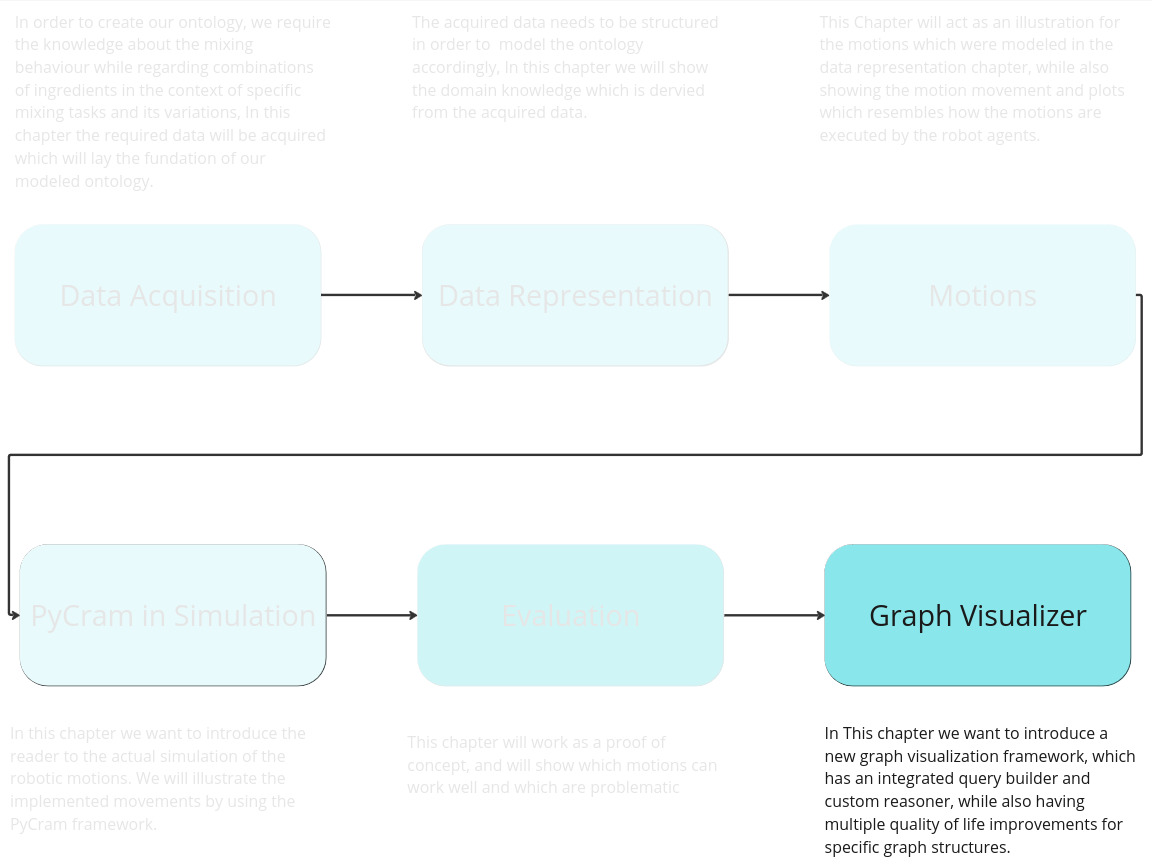
\includegraphics[scale=0.3]{Graphics/overview_6.jpg}
\end{figure}
During the process of working on the master's thesis, we were searching for a framework that could visually represent our implemented knowledge graph. Our aim was to clarify the connections and relationships between individual classes. In our search, we found several interesting frameworks that seemed suitable for our needs, which are also mentioned in the \nameref{chap:Related_work} chapter.

However, these solutions weren't entirely satisfactory for us because they lacked some features that we deemed important. Therefore, we decided to develop our own framwework, which should serve as a good visualization framework for our and similar use cases.

In this chapter, we present the framework we developed, from the initial idea to the implementation and the functionalities of our tool.

\section{Main concept}
\label{sec:MainConceps}

We decided on 3 main components that the new framework should include:
\begin{itemize}
    \item Clear Visualization: Our first goal was to facilitate navigation through the knowledge graph by highlighting the relations and classes of the graph as clearly as possible. This could be achieved, for example, by using different colors for different classes or by highlighting a class and its associated classes to which a relation exists. Additionally, we aim to make the graph as clear as possible and reduce the number of nodes to those that are ultimately essential for visualization.
    \item To clarify the relations between the queries, we implement a query builder that, given a class, can point to other classes through the relation, which in turn can point to further classes through another relation, as long as the user desires or there are no further relations. This should be done without having to use the SPARQL query language, making it much easier for the user. The Query Builder outputs a filtered graph with the selected triples.
    \item Inference Query: Since a part of our work relies on inferences, we want to implement an inference query that can indicate inferred parameters based on the input of certain classes. This use case is quite specific to our scenario, but it should also be able to map to other ontologies. The output should be an action tree with the inferred parameters and a visualized graph with the associated classes that play a role in the inference.
\end{itemize}

\section{Architecture}
\label{sec:Architecture}

The architecture consists of a full-stack framework, utilizing \textit{flask} as the web framework in the backend and \textit{HTML} and \textit{JavaScript} for the frontend. 
We use a modified version of \textit{bootstrap} for styling the \textit{HTML}-pages. Additionally, in the backend, we utilize the \textit{rdfLib}(section not yet written, 
\ref{sec:Libraries}) library to process data from the knowledge base. The \textit{JavaScript} functions are responsible for visualizing the graph, which is done using the \textit{vis.js}(section not yet written, 
\ref{sec:Libraries}) library. The following graphics are intended to visually represent a simple description of the architecture, as well as display the folder structure.
\begin{figure}[H]
    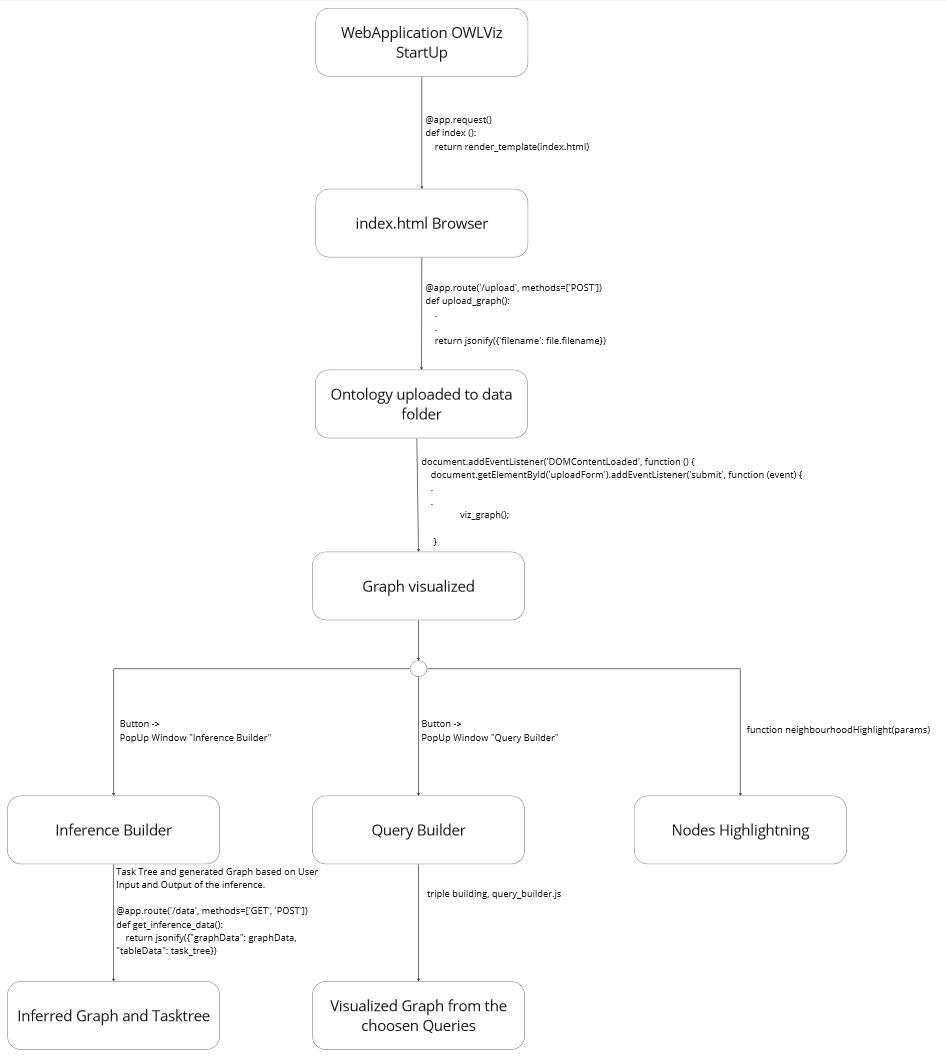
\includegraphics[scale=0.35]{Graphics/OWLViz_architecture.jpg}
    \label{fig:OWLViz_architecture}
    \caption{Architecture chart for the OWLVisualizer framework}
\end{figure}

\dirtree{%
.1 main.py.
.1 templates.
.2 index.html.
.1 data.
.1 static.
.2 graphviz.js.
.2 query\_builder.js.
.1 src.
.2 graph.
.3 graph.py.
.3 coloring.py.
.3 graph\_utility.py.
.2 inference\_builder.py.
.2 query\_builder.py.
}
Below, we want to take a closer look at the individual points of the architecture from a top-level perspective.

\subsubsection{WebApp StartUp} 

To start the application, the Python script \textit{main.py} has to be executed. This can be done using the following command, provided that the necessary libraries have been installed:
\textit{\$: python main.py}

This will start the \textit{flask} web application and open the homepage \textit{index.html}.
\begin{figure}[!ht]
    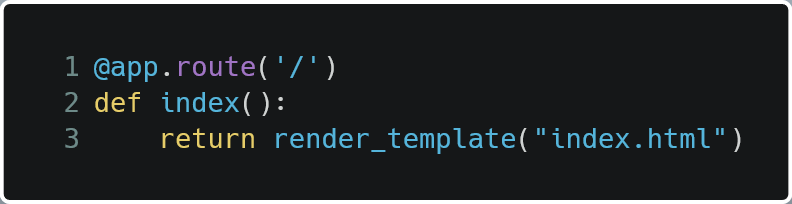
\includegraphics[scale=0.35]{Graphics/def_index.png}
    \caption{\textit{index()} - function.}
\end{figure}

\begin{itemize}
        \item \textit{@app.route("/")} indicates which function is executed first when the framework is started.
        \item \textit{render\_template("index.html")} indicates which \textit{HTML} page is being called, in this case, \textit{index.html}.
\end{itemize}

\subsubsection{Upload Ontology}

The web app initially starts with a (almost) blank \textit{HTML} page, which only contains a navigation bar. 
\begin{figure}[H]
    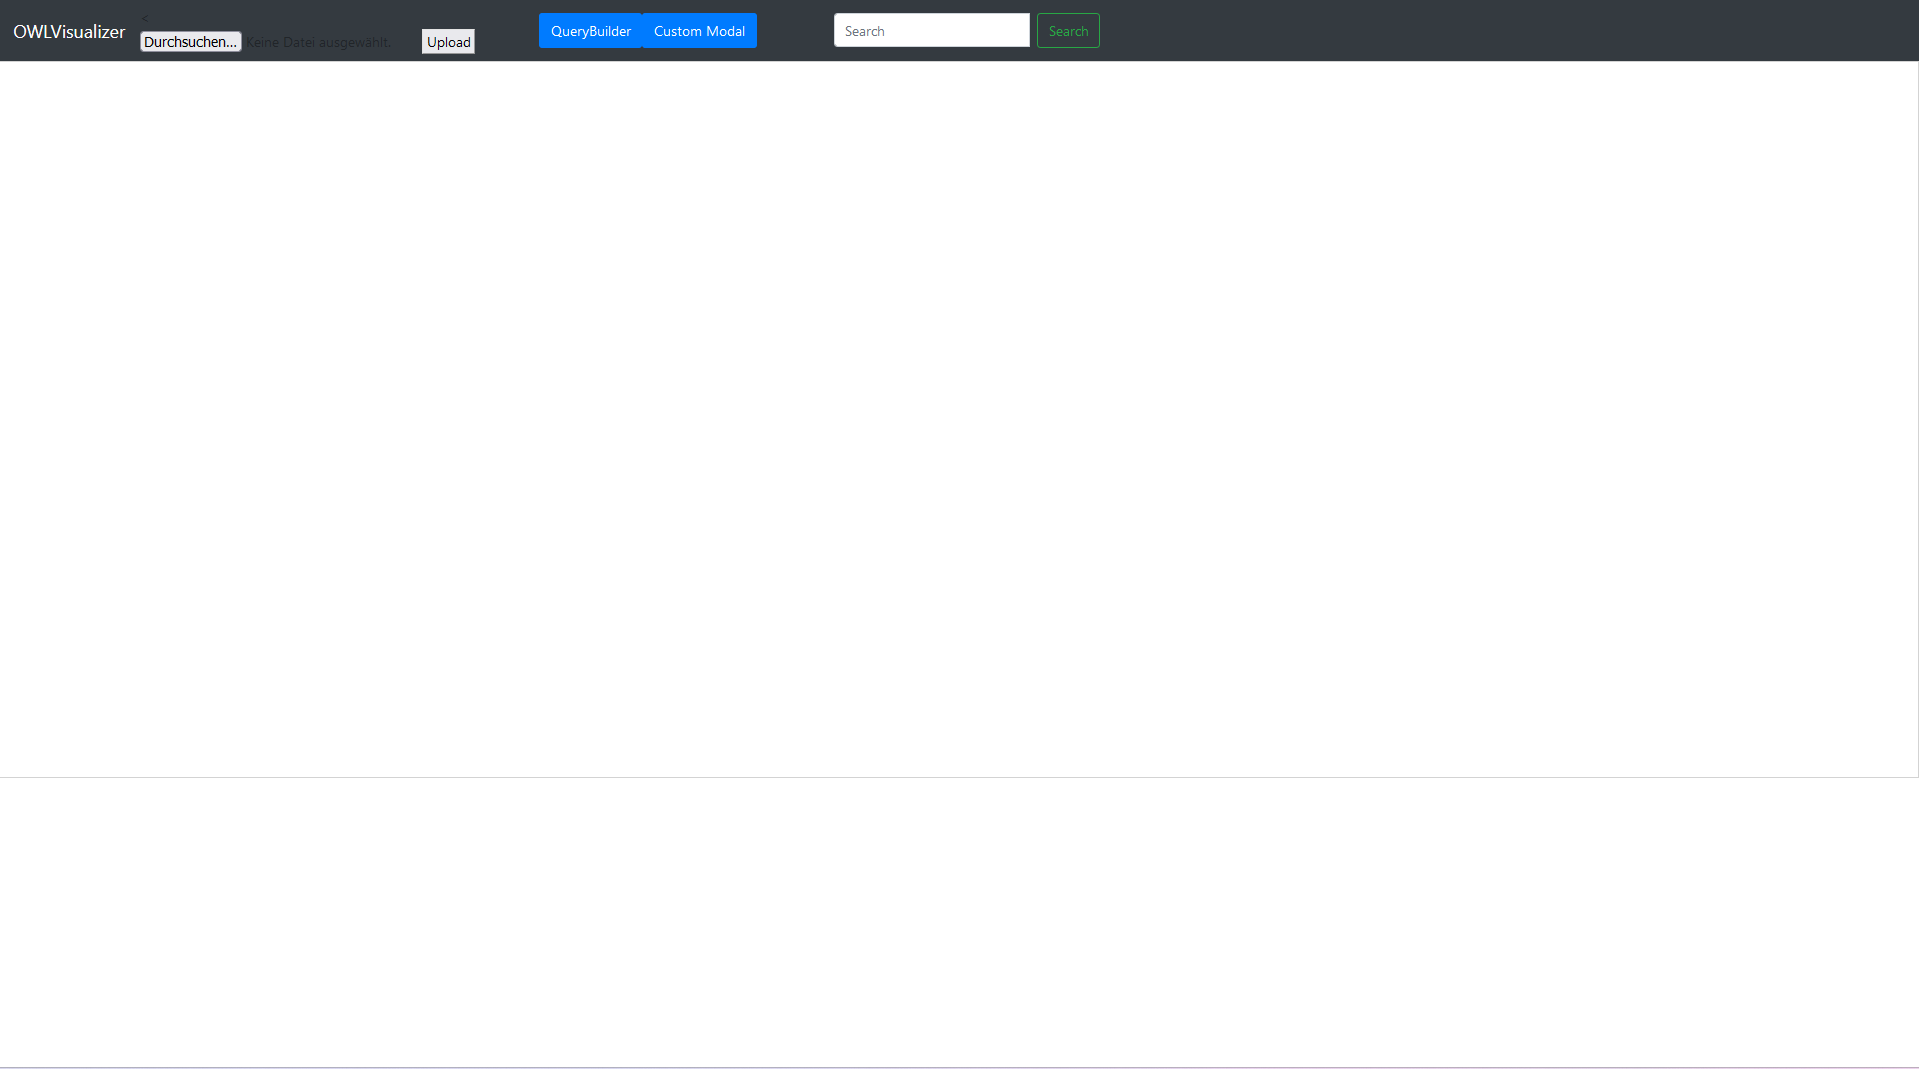
\includegraphics[scale=0.3]{Graphics/webapp_startupt_html.png}
    \caption{Startpage of the framework}
\end{figure}

Now, the user has the option to upload an ontology to work with. The function \textit{upload\_graph()} saves the ontology in the \textit{data} folder.

\begin{figure}[H]
    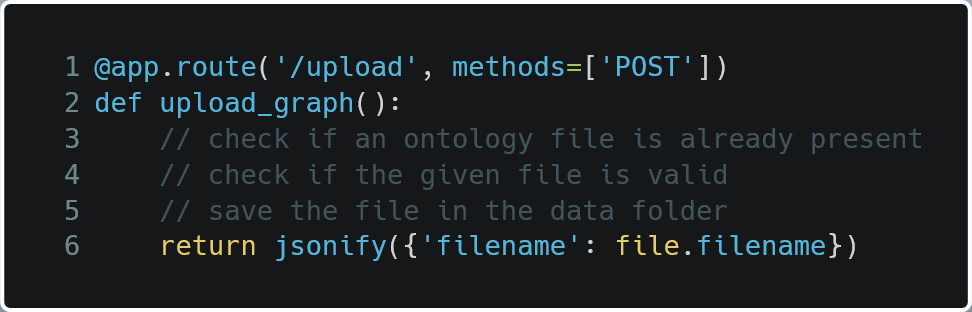
\includegraphics[scale=0.2]{Graphics/upload_graph.png}
    \caption{\textit{upload\_graph()} - function.}
\end{figure}

\subsubsection{Visualized Graph}
Once the ontology has been uploaded, the \textit{JavaScript} function \textit{viz\_graph()} is executed, 
which ultimately visualizes the graph. This function fetches the required sets of nodes and edges from the backend function \textit{get\_graph\_data()}.

\begin{figure}[H]
    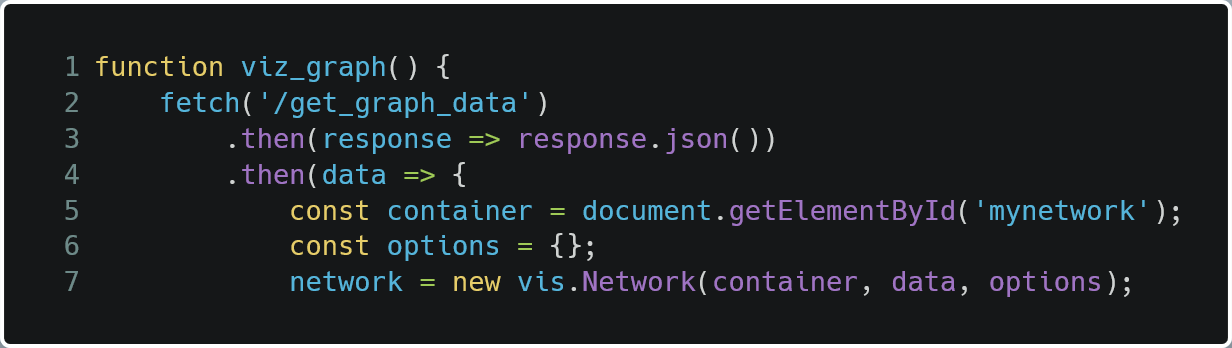
\includegraphics[scale=0.2]{Graphics/viz_graph_function().png}
    \caption{\textit{viz\_graph()} - function.}

\end{figure}

\begin{figure}[H]
    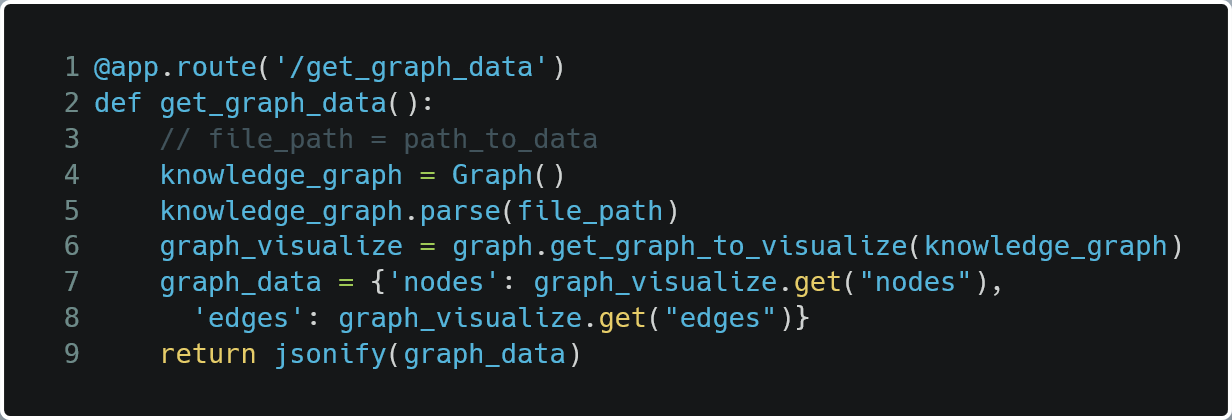
\includegraphics[scale=0.2]{Graphics/get_graph_data.png}
    \caption{\textit{get\_graph\_data()} - function.}

\end{figure}

The data processing is complex and will be further elaborated in the \nameref{sec:Implementation} section. 
Additionally, we have written a section intended to provide a simple introduction to our framework, which can be found in the section 
\nameref{sec:Introducing the framework with a trivial example} . This section aims to illustrate the functionality through a trivial example.
\subsubsection*{Nodes Highlightning}

For large graphs, it can become difficult to maintain an overview of the nodes and their associated relations. 
Therefore, we are implementing a function that highlights a node as well as its neighboring nodes. 
This is intended to make it easier to understand the relationships between a class and its associated nodes. 

The required function is a \textit{JavaScript} function that takes a clicked node as a parameter and calculates its neighboring nodes based on that. 
Subsequently, all nodes are grayed out, and the selected node and its neighbors are restored to their original color. This makes the selected nodes appear "highlighted".

\begin{figure}[H]
    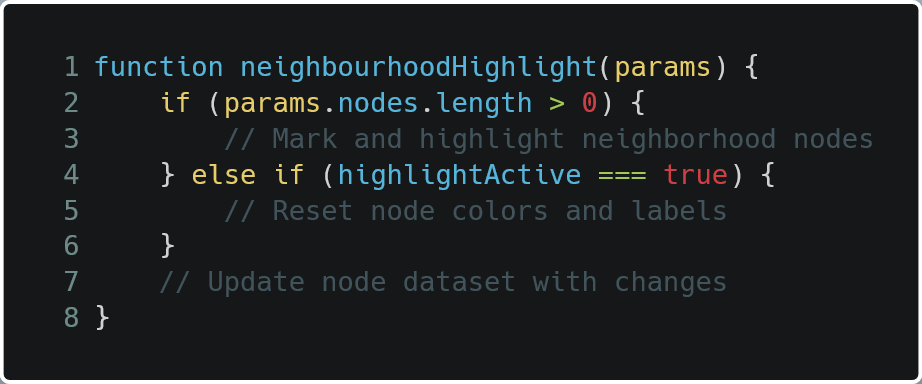
\includegraphics[scale=0.25]{Graphics/neighbourhood_highlighting.png}
    \caption{\textit{neighbourhoodHighlight()}-function}
\end{figure}

Here is an example of a graph with highlighted nodes:

\begin{figure}[H]
    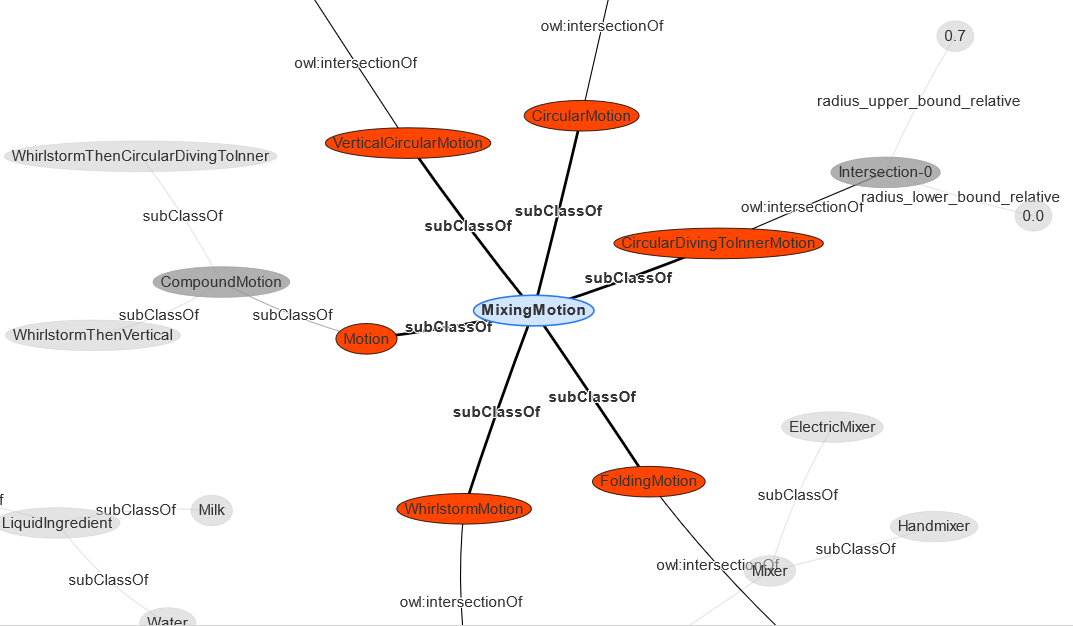
\includegraphics[scale=0.3]{Graphics/nodes_highlight_html.png}
    \caption{graph with highlighted nodes}
\end{figure}

\subsubsection{Query Builder - Naser}
The \textit{QueryBuilder} is another feature of the OWLVisualizer. Its core feature is making triple matching possible without possesing knowledge of  
constructing SPARQL queries. Next to triple matching, visualizing selected triples is made possible, to further visualize relationships between concepts and restrictions
and instances. 
Class restrictions in particular are easily queried using the QueryBuilder, without knowing how to actually query them. 

Another functionality is to construct a SPARQL query from the matched triples for further usage of the user. 

In this section the requirements for this feature are explained.

\paragraph{Requirements}

The \textit{QueryBuilder} needs a processable graph to apply the pattern matching on. 
Two different sources of data can be considered. The parsed graph from rdflib or the graph model for visualization.
Choosing the graph model for visualization is rational since we introduce consistency between graph visualization and
triple matching in the \textit{QueryBuilder}. The main drawback of choosing the graph visualization model is, constructing a
SPARQL query from this model instead of the rdflib parsed graph is made difficult since the graph has to be detransformed into the rdflib parsed graph, to then construct the 
SPARQL query. How this is handled will be discussed in a seperate paragraph. 


\paragraph{Triple Matching}
The concept of triple matching for the \textit{QueryBuilder} is rather simple.
Consider a triple consisting of subject, predicate and object.
A subject is connected via a set of predicates to a set of objects. 
For example we have a subject \textit{A} which has predicates ${\textit{subClassOf}, \textit{equivalentClass}}$
available objects are ${\textit{B}, \textit{C}, \textit{D}}$, where A is a subClassOf B and A is equivalent to C and D. 
Suppose A is picked, then available predicates are ${\textit{subClassOf}, \textit{equivalentClass}}$.
If \textit{subClassOf} is chosen available objects are \textit{B}.
In essence the QueryBuilder is doing exactly that.



\paragraph{Initial Triple Matching}
There is no complete triple matching available if no triples have been selected yet. For example class restrictions are not queryable, they will be queryable once a class
with restrictions has been selected. Initial triple matching is applied to OWL-Classes and instances.

\paragraph{Base Triple Matching} 
Once a triple has been selected more options are available. 
If a OWL-Class has been chosen, the following triples become available:
Relationships with classes connected with subClassOf or equivalentClass.
Classes with class restriction. 
Classes and their instances. 

If an instance has been picked, relationships between other instances are available
between attributes and to which class this instance belongs is available too.

\paragraph{Graphfiltering}
Based on the matched triples provided by the user, the model for graph visualization filtered based upon 
the matched triples to visualize it. The filtered graph contains all information used in the graph visualization in 
the web app to ensure that the view or partial view remains consistent with the original graph.

\paragraph{SPARQL}
To generate a SPARQL query based on the selected triples, triples containing restrictions have to be transformed back into 
rdf graph containing blank nodes. This is relevant for querying in SPARQL, since matching against blanknodes is mandatory to retrieve 
properties and values/classes out of a restriction. 

The resulting query consists off all added triples by the user, where subject, predicate and object is replaced by the 
chosen values. An exception is made for blanknodes, since their indentifiers change each time an ontology is parsed into 
a rdf graph using rdflib. Precise identification is not possible, thus blanknodes have to be replaced with variables, to 
be able to do the triple matching.







\subsubsection{Inference Builder}
The last option for the user to execute functions on a graph is the Inference Builder. 
It's important to note that the Inference Builder is not a generic use case and in this version, it's tailored to the Mixing Graph (see \nameref{chap:Data_representation}). 
In the \nameref{sec:Implementation} section, the implementation is further explained, demonstrating how it could potentially be implemented for other ontologies as well. 
In our case, we infer a motion and its corresponding parameters based on a given task and a potentially long list of ingredients. 
The Inference Builder then generates a graph that only displays the corresponding nodes for clarity, as well as a task tree that can be followed by an agent.
In the first step, the task and the ingredients are sent to the backend for inference, which in turn sends back the inferred motion and parameters to the frontend.

\begin{figure}[H]
    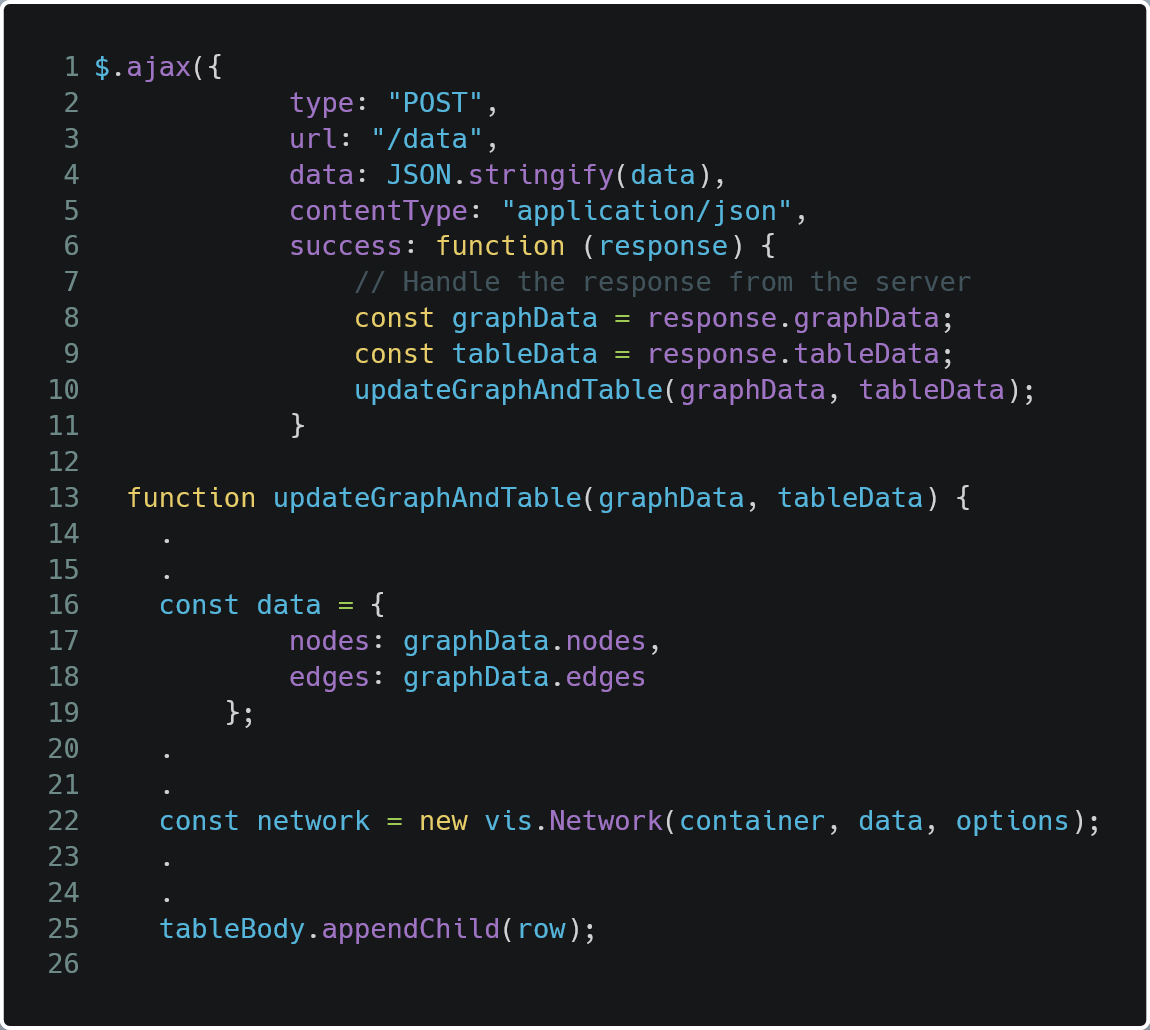
\includegraphics[scale=0.25]{Graphics/inference_builder_js.png}
    \caption{data processing for the inference builder}
\end{figure}

The backend function processes the inference with the received parameters, which are then used for visualization.

\begin{figure}[H]
    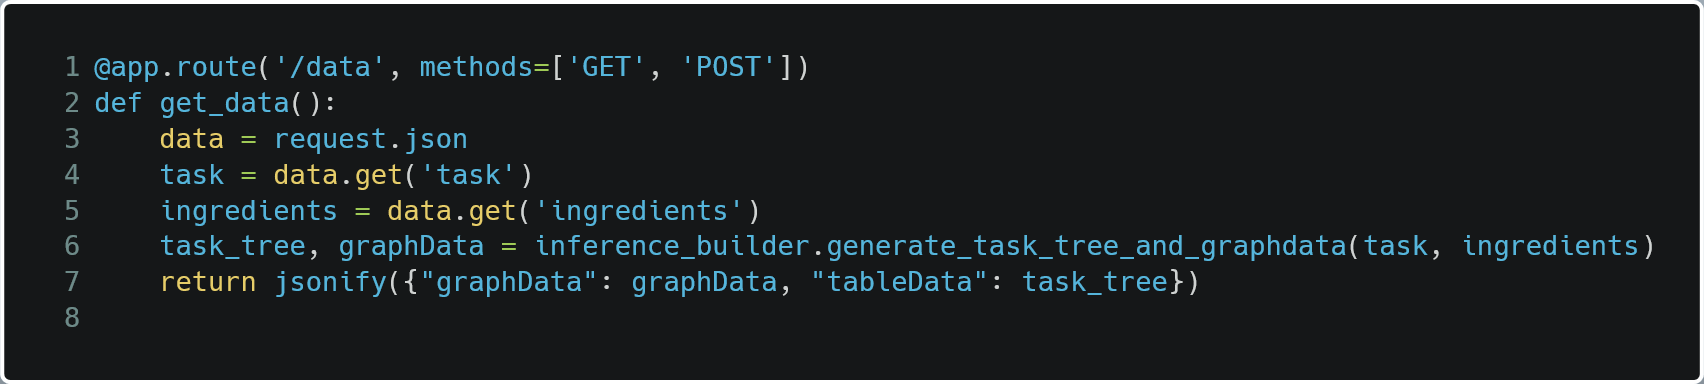
\includegraphics[scale=0.23]{Graphics/get_data.png}
    \caption{\textit{get\_data()}-function}
\end{figure}

After processing the data, the graph and the task tree are visualized based on the user input.

\begin{figure}[H]
    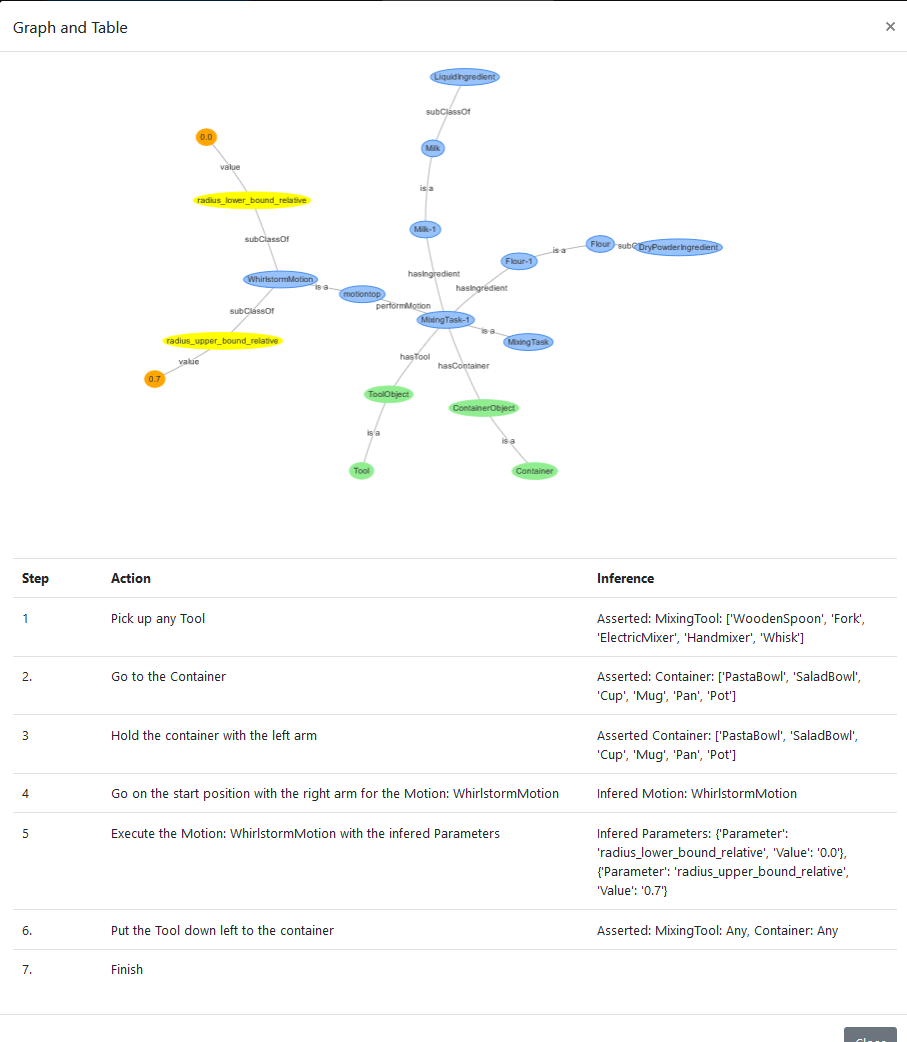
\includegraphics[scale=0.5]{Graphics/new_inference_graph.png}
    \caption{inferred graph and task tree.}
    \label{fig:graph_inferred}
\end{figure}

The data processing and the detailed implementation of the Inference Builder will be further explained in the \nameref{sec:Implementation} section.

\subsubsection{Simple Example of our framework}
\label{sec:Introducing the framework with a trivial example}
In this section, we present a simple example of our framework, from processing the ontology to visualization in the web application. This is intended to facilitate the reader's understanding of our framework. For this purpose, we create a small and simple ontology to explain the program flow in a straightforward manner. Additionally, we aim to demonstrate how this ontology is processed and what the interface between the frontend and backend looks like.

\subsubsection{Simple Ontology}

\begin{figure}[H]
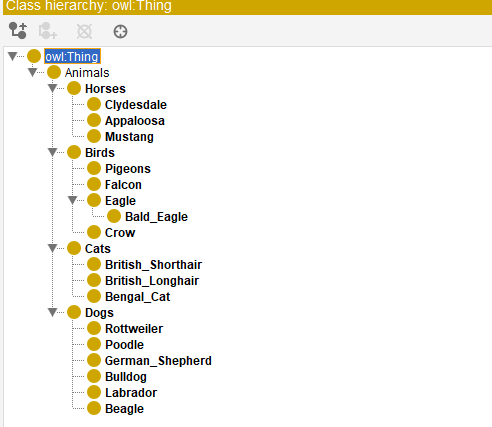
\includegraphics[scale=0.5]{Graphics/simple_ontology_owlviz.png}
\caption{Simple example of an ontology}
\end{figure}

The ontology created for this purpose aims to provide a simple representation of various animal species. It includes superclass categories such as \textit{Horses, Birds, Cats, and Dogs}, as well as subclasses like \textit{Labrador} and \textit{Beagle}, which are subclasses of the \textit{Dog} superclass. This ontology does not depict complicated relations; rather, the individual classes are only connected to each other through the \textit{subClassOf} relation.

\subsubsection{Ontology processing}
Next, the ontology is parsed. Using the \textit{rdfLib}(section not yet written, 
\ref{sec:Libraries}) library , the ontology is read and made queryable. The goal is to retrieve all classes of this ontology along with their associated relations. 
These are then stored in a list, which will be important for visualizing the graph in the frontend.
\begin{figure}[H]
    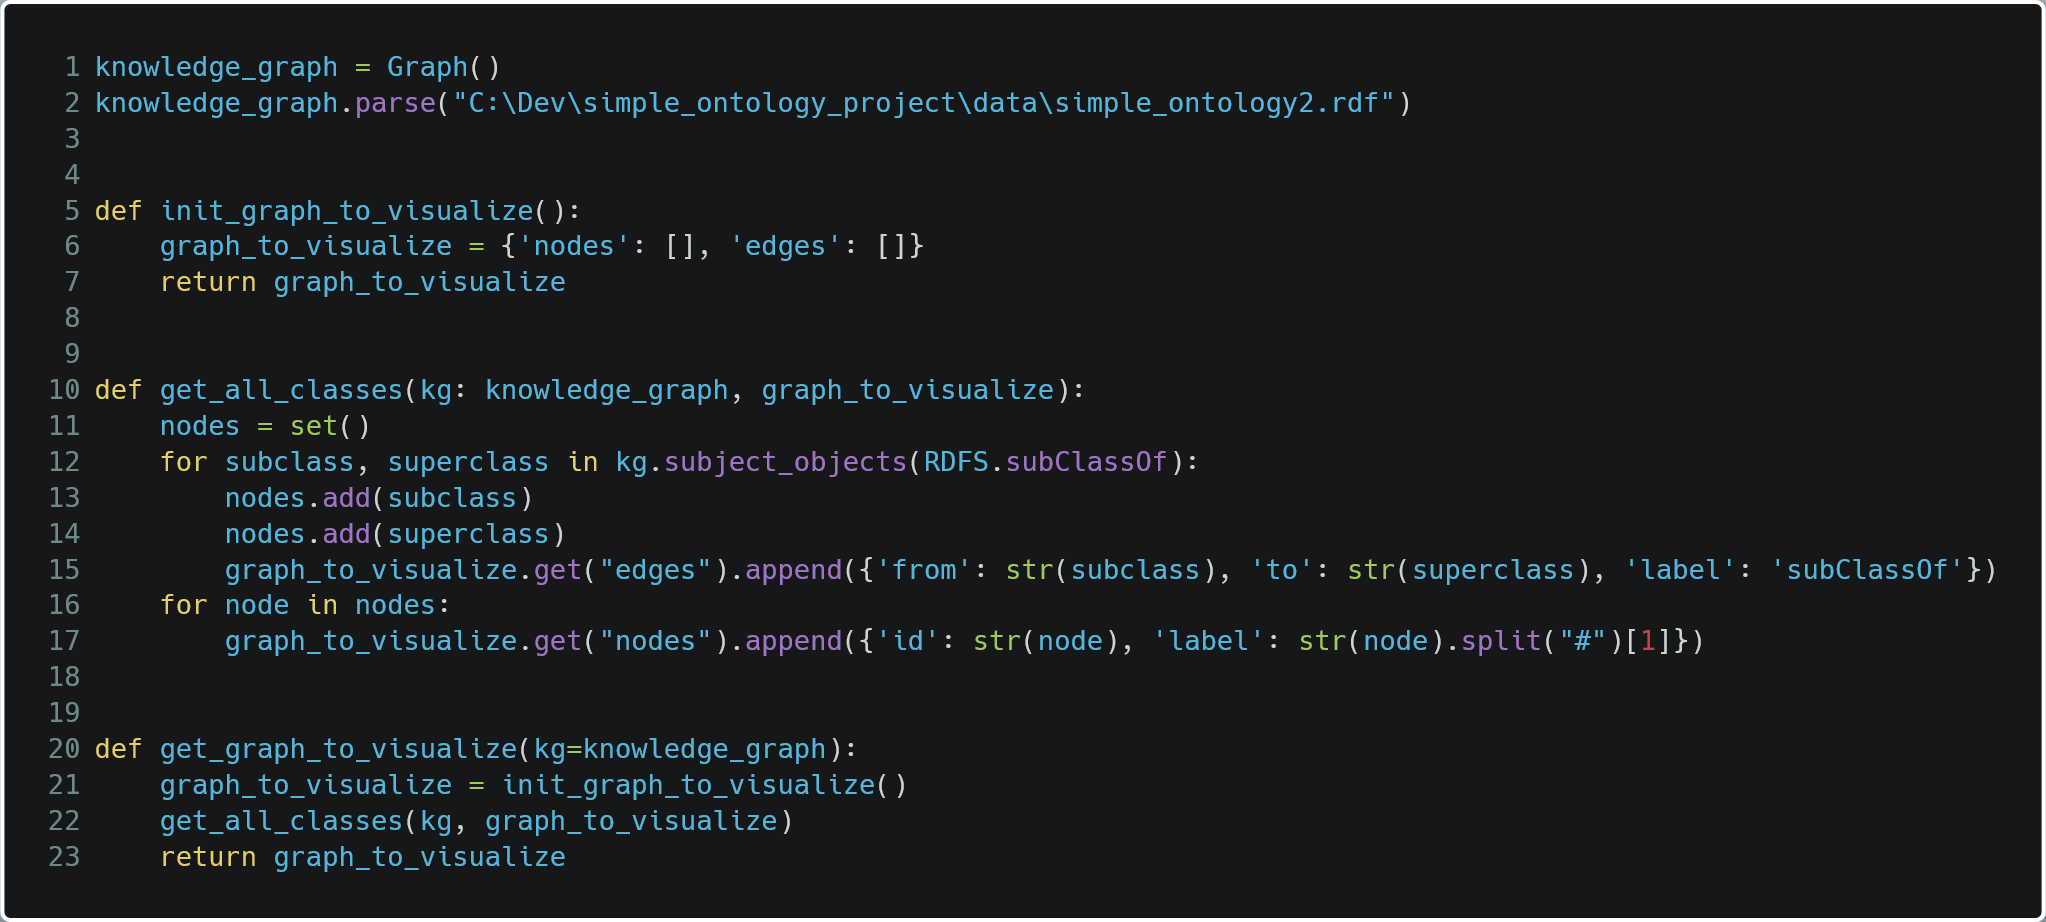
\includegraphics[scale=0.2]{Graphics/simple_ontology_graph_init.png}
    \caption{Graph initialisation}
    \end{figure}
    
\begin{itemize}
    \item Lines 1 and 2: A graph is created, and the ontology is parsed and inserted into this graph.
    \item Lines 5 to 7: This function serves to pass on the set of nodes and edges for the visualization of the graph. The nodes represent the classes, while the edges represent the relations.
    \item Lines 10 to 17: This function searches the graph for all classes, which are distinguished between superclass and subclass. The edges then point from a superclass to its corresponding subclass. Both classes are also added to a list of nodes.
    \item Lines 20 to 23: The set of nodes and edges is initialized for the graph and is now ready for visualization.
\end{itemize}

With that, the processing of the ontology for the set of nodes and edges for visualization has been completed. Now, we want to visualize these sets.

\subsubsection{From Backend to FrontEnd: Visualization}

As a reminder: The framework we are using is \textit{flask}, which facilitates communication between the frontend, consisting of \textit{HTML}, \textit{CSS}, and \textit{JavaScript}, 
and our backend, where the graph is prepared for visualization. First, we'll explain the communication with the frontend.

\begin{figure}[H]
    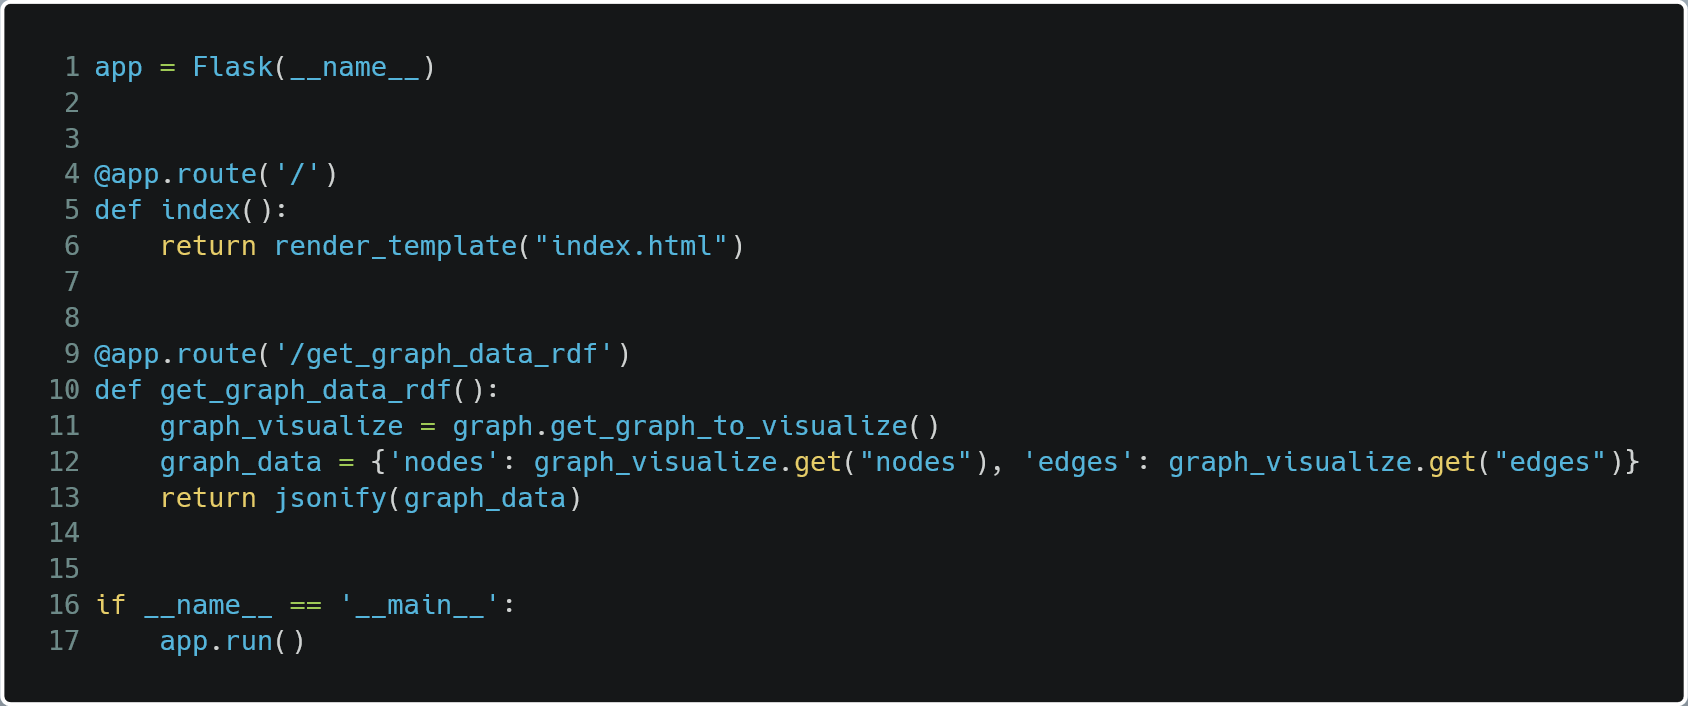
\includegraphics[scale=0.2]{Graphics/simple_ontology_flask.png}
    \caption{Interface between Front and BackEnd}
    \end{figure}
    
\begin{itemize}
    \item Lines 1 to 6: When the application starts, the \textit{HTML} page \textit{index.html} is called.
    \item Lines 9 to 17: When the function \textit{get\_graph\_data\_rdf} is called, the set of nodes and edges is retrieved in a format that can be processed by the \textit{JavaScript} library \textit{vis.js}.
\end{itemize}

The function \textit{get\_graph\_data\_rdf} is called in the frontend \textit{JavaScript}.

\begin{figure}[H]
    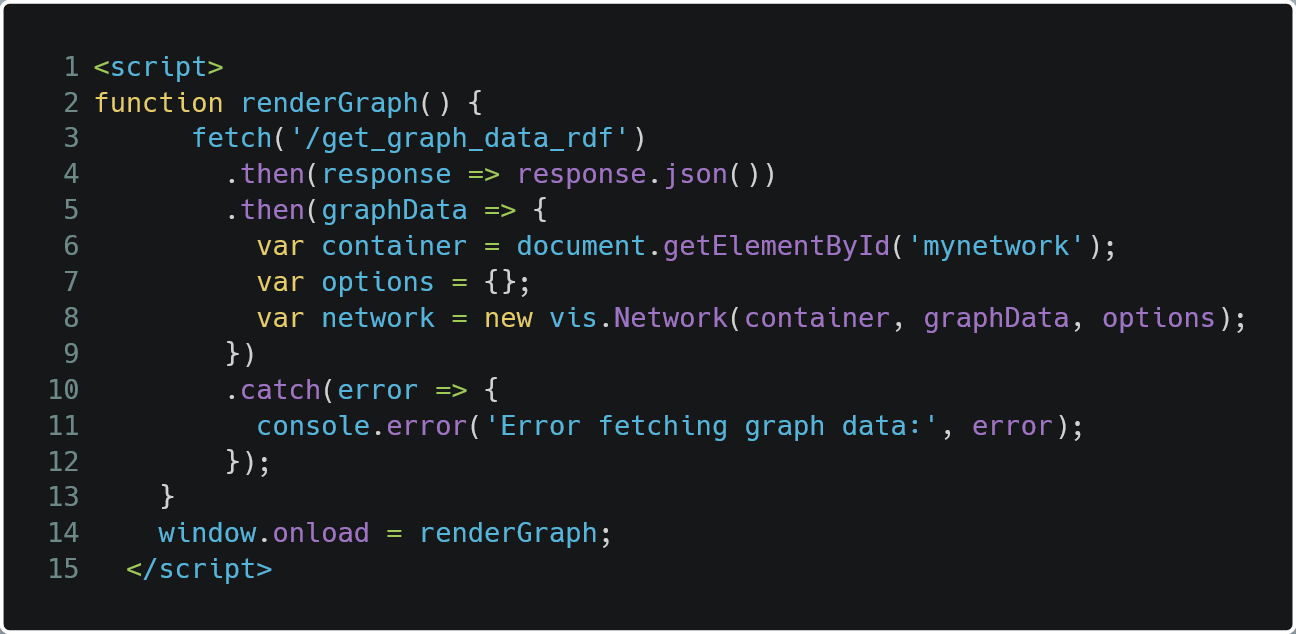
\includegraphics[scale=0.23]{Graphics/simple_ontology_js.png}
    \caption{trivialized example of the FrontEnd}
    \end{figure}

The graph is created using the data extracted from the output of the function 
\textit{get\_graph\_data\_rdf}. In line 14, it is specified that the function for rendering the graph is called directly upon loading the \textit{HTML} page.

\begin{figure}[H]
    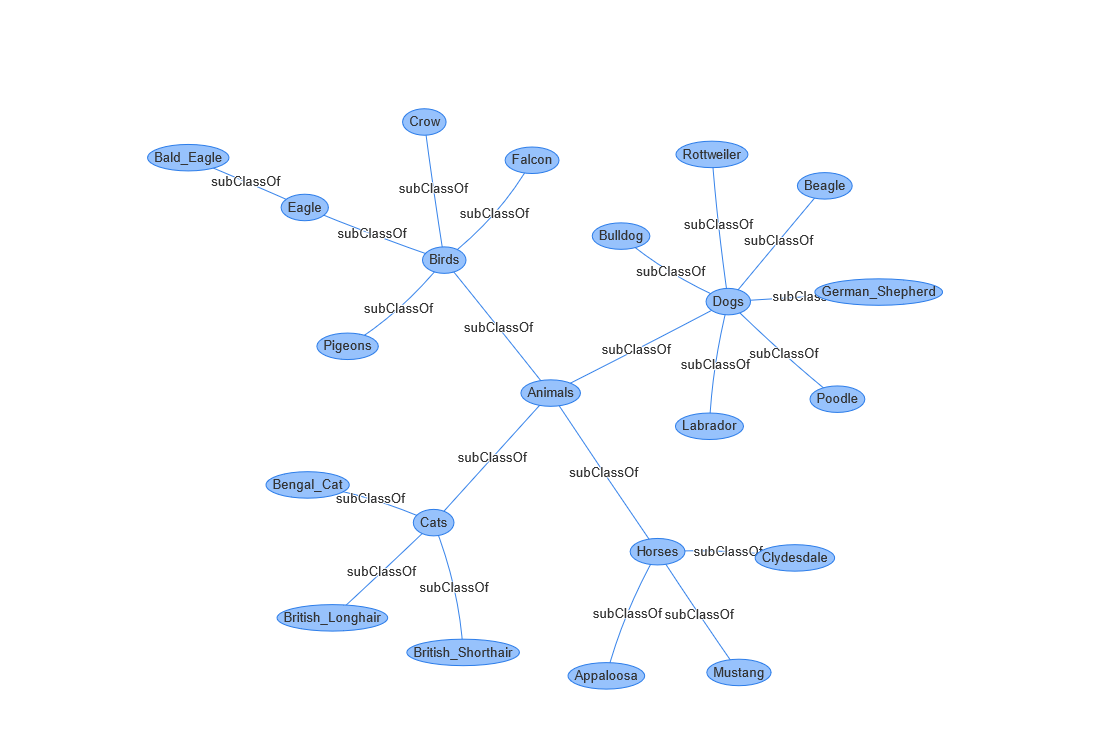
\includegraphics[scale=0.45]{Graphics/simple_graph.png}
    \caption{generatd example-graph}
\end{figure}


This example illustrated the process of visualizing a simple ontology. However, the ontologies we tested during the implementation were much more complex and required various specific implementations to visualize them. Additionally, we made several improvements to the visualization itself compared to the standard graph. The implementation of the backend, as well as the three different functions (see \nameref{sec:MainConceps}), will be described in more detail in the next section.
\section{Implementation}
\label{sec:Implementation}

This section explains the detailed implementation of the framework and highlights the challenges and solutions encountered during implementation. In the previous section, we provided a trivial example intended to serve as an introduction for users to understand the framework's basics. However, since ontologies can vary in structure and some relations can be complex, a simple implementation may not suffice in most cases.

We will begin by explaining the implementation of the backend, and towards the end of the section, we will also address some aspects of the frontend. In the conclusion, we will touch upon points that, in our opinion, could be implemented in the future and discuss any problems/limitations this framework might have.
\subsection{BackEnd}

As explained in the \nameref{sec:Architecture} section and demonstrated in the Introductory Example section (see: \nameref{sec:Introducing the framework with a trivial example}), the framework uses \textit{flask} as its backend interface. 
This ultimately serves to send processed data to the frontend or receive data from it. Now, we'd like to explain how this data is processed and how it has been adequately prepared.
\subsubsection{Graph Verarbeitung - Work in Progress}

To visualize a graph using the JavaScript library \textit{vis.js} (NOTE), we need a set of nodes and edges. An example of how these could be processed was explained here (NOTE). The existing classes of an ontology are not always connected only by the \textit{subClassOf} relation. Some relations pose challenges in the graph because lists of possible classes related to a superclass can also appear. This poses a problem for visualization because in such cases, so-called \textit{Blank Nodes} appear. These nodes do not represent any information but merely serve as connection nodes between 2 or more classes. These nodes are connected by relations such as \textit{owl:intersectionOf}, \textit{owl:first}, or \textit{owl:rest} and have no added value for our visualization. The first challenge was to adequately process these nodes to remove \textit{Blank Nodes} from the visualized graph and to represent the correct relation between the classes between which these \textit{Blank Nodes} existed

\subsubsection{Implementation of the Query Builder - Work in Progress}


\subsubsection{Implementation of the Inference Builder}
As described in the \nameref{sec:Architecture}, the Inference Builder is intended to visualize and organize the results of inference within the ontology. 
The inference refers to defined \textit{SWRL} rules (see: \nameref{sec:SWRL}), which can then be queried using the \textit{OWLReady2} library (see: \nameref{sec:OWLReady}).
Therefore, the implementation assumes this type of rules. The rules implemented by us were explained in the \nameref{chap:Motions} chapter. 
Ultimately, the goal is to execute the inference based on user input and visualize the results.
\paragraph{User Input}

The user selects a task and any number of ingredients.
\begin{figure}[H]
    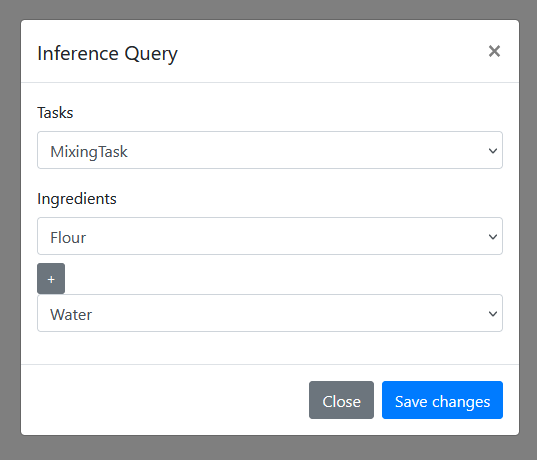
\includegraphics[scale=0.45]{Graphics/inference_user_input.png}
    \caption{Select fields for the inference.}
\end{figure}
These data are extracted from the ontology using the \textit{rdfLib}(section not yet written, 
\ref{sec:Libraries}). The following code will explain this further.

\begin{figure}[H]
    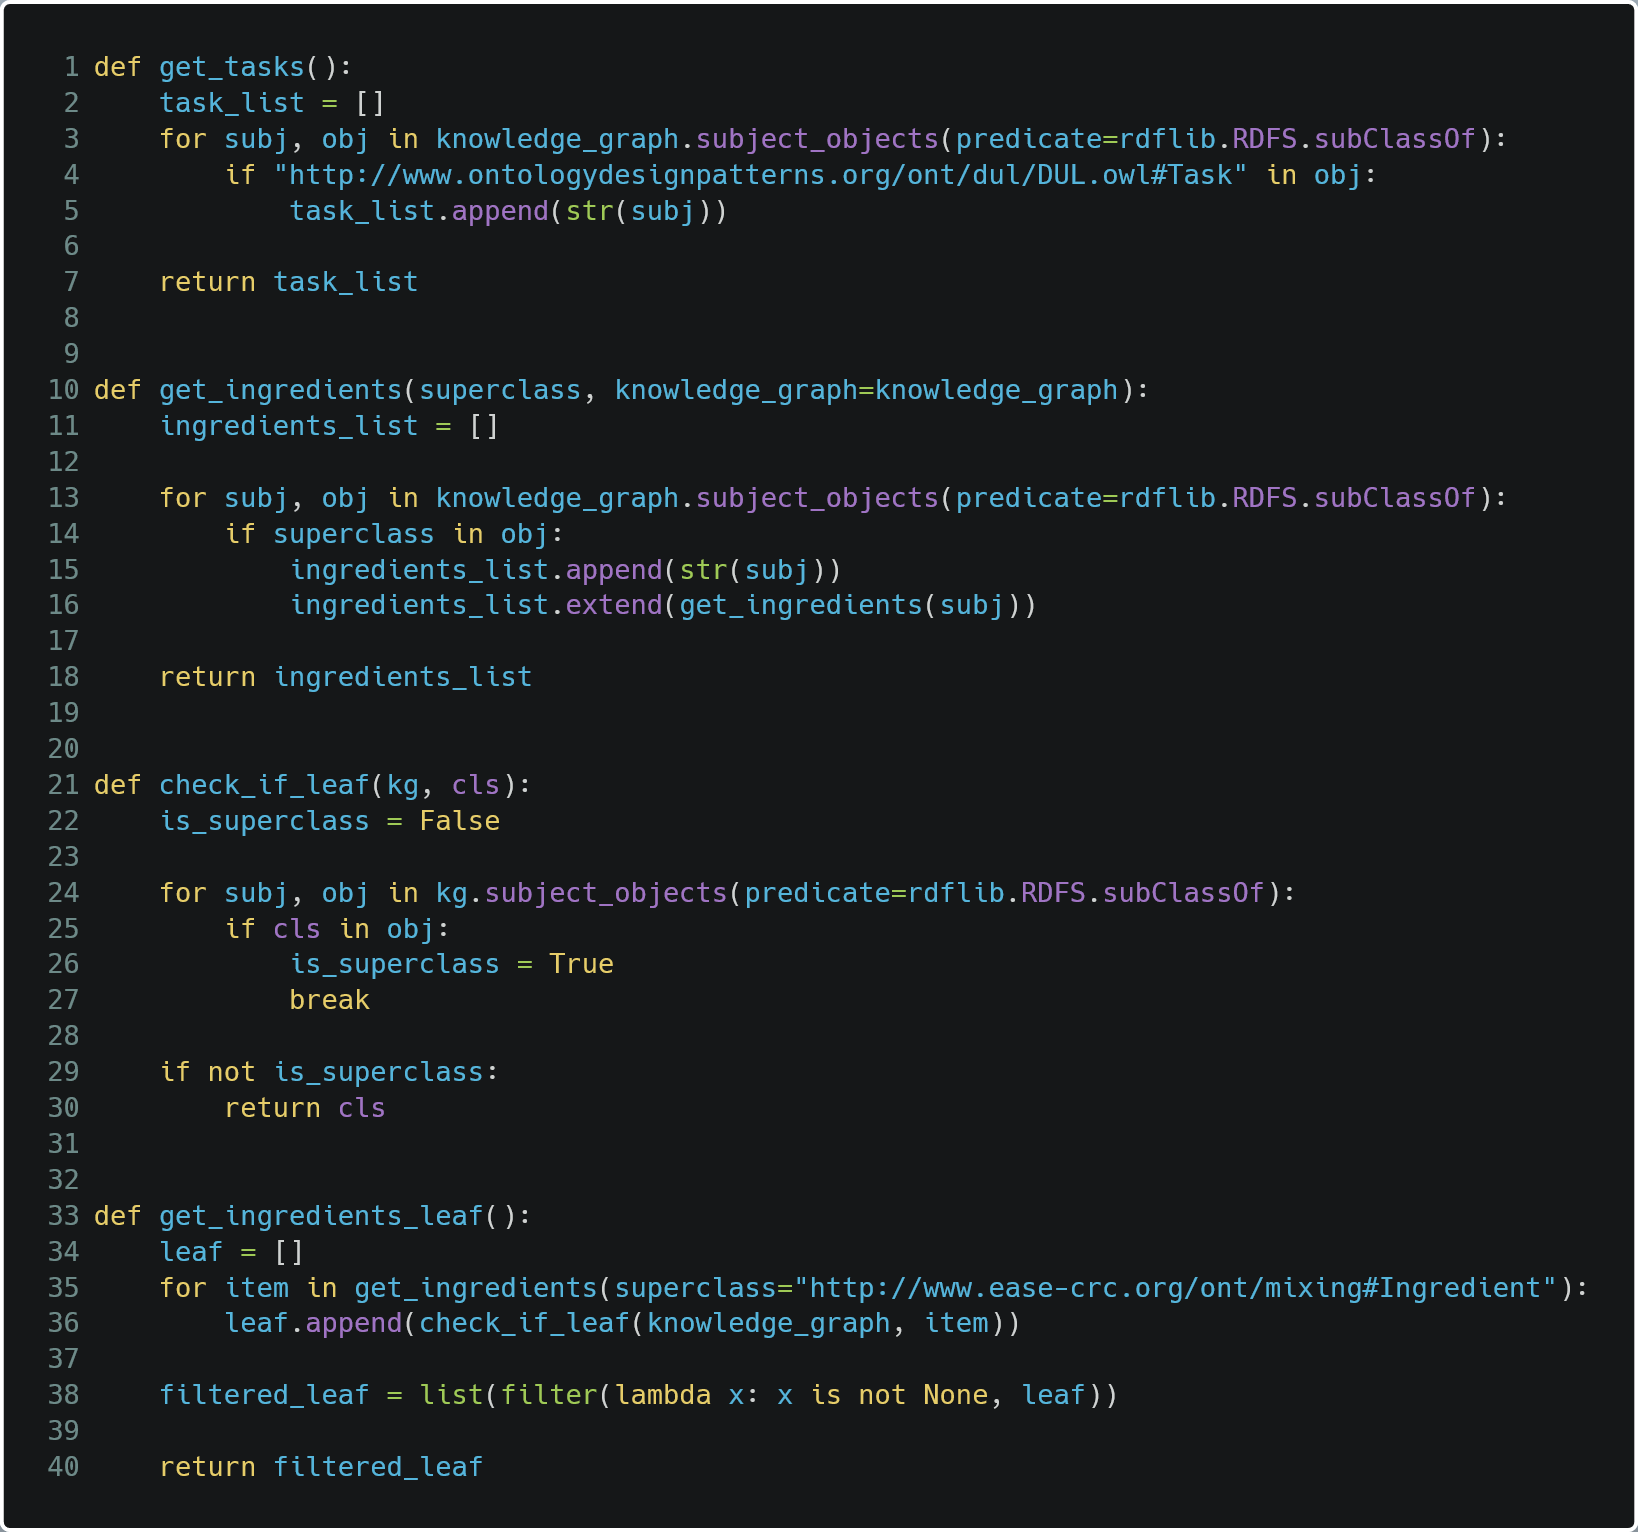
\includegraphics[scale=0.22]{Graphics/get_tasks_ingredients.png}
    \caption{Code snippet for querying the tasks and ingredients from the ontology}
\end{figure}

\begin{itemize}
    \item Lines 1 - 7: Each triple where the predicate of the relation matches \textit{subClassOf} is queried. Additionally, it checks whether the object corresponds to the class \textit{Task}. These elements are then added to a list, which is also returned.
    \item Lines 10 - 18: Similar to the above function, the subclasses of ingredients are returned. The only difference is that the function is called recursively since the class \textit{Ingredients} has subclasses at multiple levels. Therefore, it also checks which class has no more subclasses.
    \item Lines 21 - 30: This function checks whether a given class corresponds to a leaf in a graph, meaning this class itself has no subclasses.
    \item Lines 33 - 40: This function ultimately returns the list of ingredients available for the user's selection.
\end{itemize}

These data are sent to the frontend using the following function:

\begin{figure}[H]
    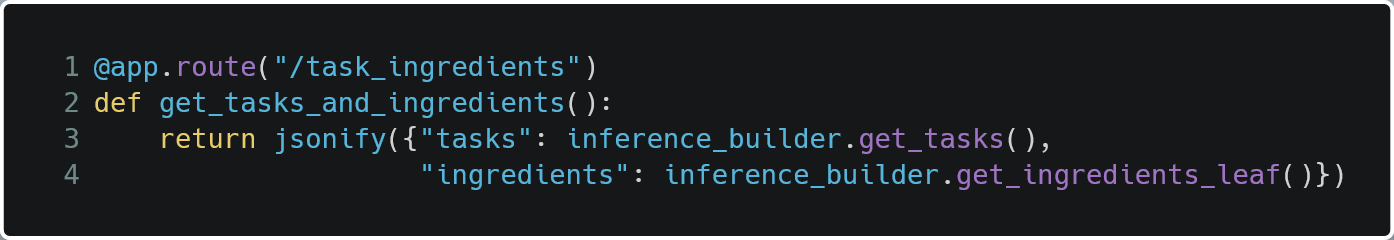
\includegraphics[scale=0.25]{Graphics/inference_main.png}
    \caption{\textit{get\_tasks\_and\_ingredients()}-function}
\end{figure}

The previously described functions are called, and the data is sent to the frontend in \textit{JSON} format. In the frontend, this data is fetched and processed.

\begin{figure}[H]
    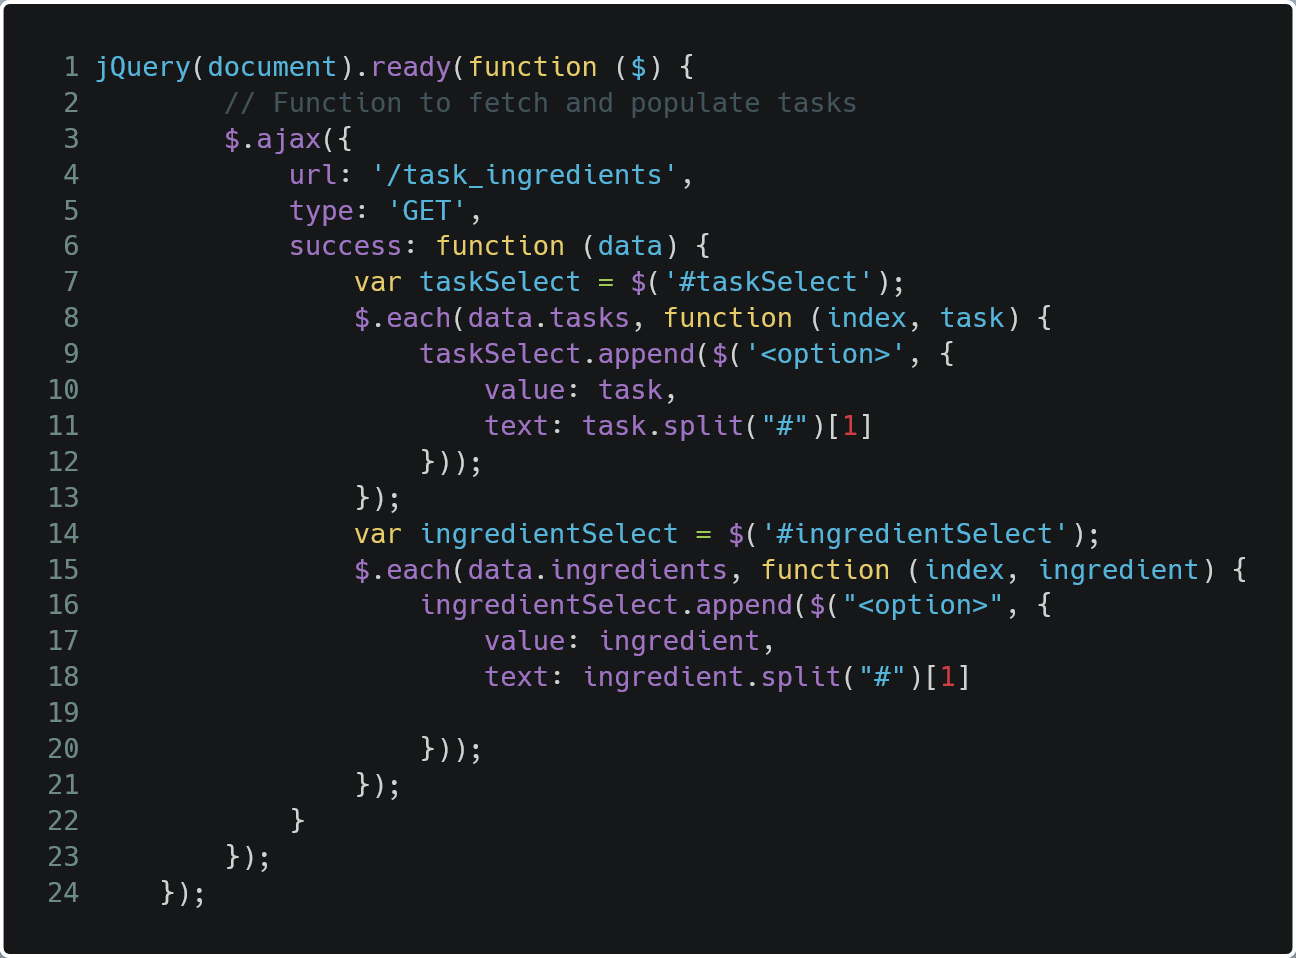
\includegraphics[scale=0.22]{Graphics/inference_frontend_fetch.png}
    \caption{Data is fetched in the FrontEnd}
\end{figure}

This function populates the entries of the select fields for task and ingredient selection with the data from the backend. 
By doing so dynamically, it ensures that even if the ontology has new entries in these classes, they will always be available for the user's selection.

\paragraph{Inference}
\label{par:Inference}

An example can illustrate the process of inference calculation. Taking the above example (see: \ref{fig:graph_inferred}), we have the input task: \textit{MixingTask} and the ingredients: \textit{Flour} and \textit{Water}. 
These two ingredients correspond to the superclasses \textit{DryPowderIngredient} and \textit{LiquidIngredient}, respectively (see: \nameref{chap:Data_representation} for more information 
about the structure of the ontology.). This combination ultimately corresponds to the \nameref{sec:SWRL}-Rule:
\begin{lstlisting}
MixingTask(?x) ^ DryPowderIngredient(?ing1) ^ hasIngredient(?x, ?ing1)
^ LiquidIngredient(?ing2) ^ hasIngredient(?x, ?ing2) ^ Motion(?motion) 
^ performMotion(?x, ?motion) -> WhirlstormMotion(?motion)
\end{lstlisting}

From this, the motion \textit{WhirlstormMotion} is inferred with the corresponding parameters:
\begin{lstlisting}
    radius_lower_bound_relative  0.0
    radius_upper_bound_relative  0.7
\end{lstlisting}
To calculate this inference, we use the library \textit{OWLReady2} (see: \nameref{sec:OWLReady}), which enables us to utilize a reasoner for the inference.
\begin{figure}[H]
    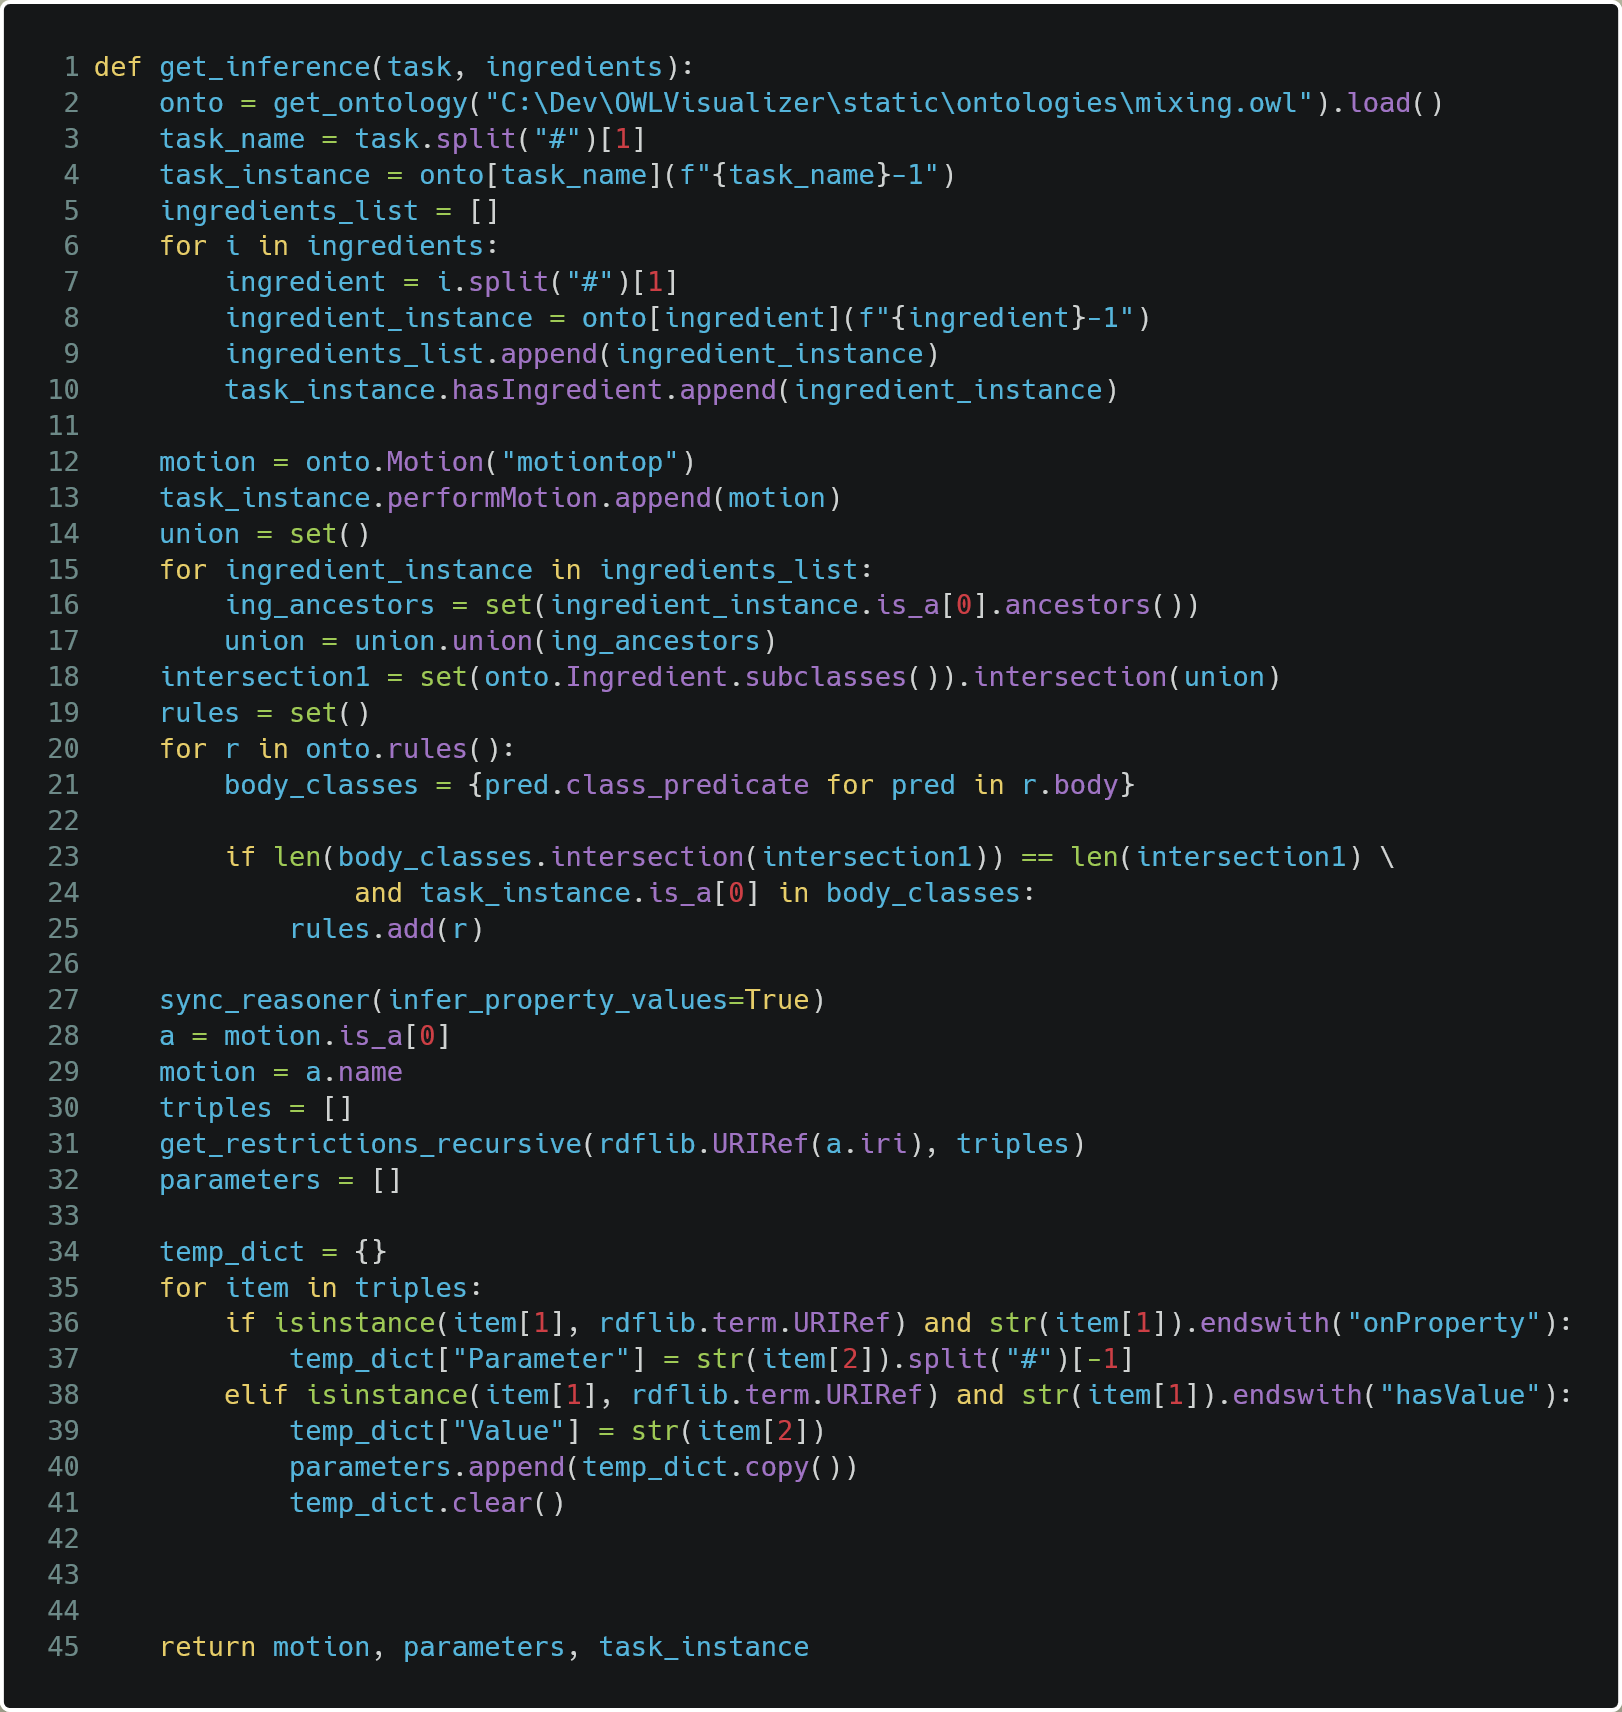
\includegraphics[scale=0.23]{Graphics/get_inference.png}
    \caption{Inference function}
\end{figure}
\begin{itemize}
    \item Lines 1 - 10: The classes are instantiated. The function takes parameters \textit{task}, corresponding to a task, and \textit{ingredients}, corresponding to a list of ingredients. In line 2, the ontology for the \textit{OWLReady2} library is instantiated to utilize the reasoner. In lines 3 and 4, the \textit{task} is instantiated. Since the task comes as input in the full \textit{IRI} format, it needs to be processed first. From lines 5 to 10, the same is done analogously for the ingredients, this time only for a list of ingredients. Subsequently, the instances of the \textit{ingredients} are added to the instance of \textit{task}.
    \item Lines 12 - 13: A top-level \textit{Motion} is instantiated to indicate that the \textit{Motion} is inferred during reasoning. ???
    \item Lines 14 - 18: Since the superclasses of the \textit{ingredients} are important for the rules, they are added to a set which will be used later for inference.
    \item Lines 19 - 25: The existing rules are examined and matched with the input to infer the correct \textit{SWRL} rules.
    \item Lines 27 - 45: Here, the reasoner is first started. The inferred motion is stored, and now it is about determining the required parameters based on the motion. These parameters are then stored in a dictionary. The function returns the motion, the parameters, and the instance of \textit{task}.
\end{itemize}

\paragraph{Preparing the Output}
For clarity, we have decided to reduce the graph to only the classes used in the inference. The middle node of the graph represents the task instance selected by the user. 
From this node, you can reach the other classes that are important for the inference. 
These classes correspond to the classes of the ingredients, i.e., the ingredient instances selected by the user, the inferred motion along with parameters, 
and each instance for the tools and containers, each of which can represent any possible combination if no selection has been made.
\begin{figure}[H]
    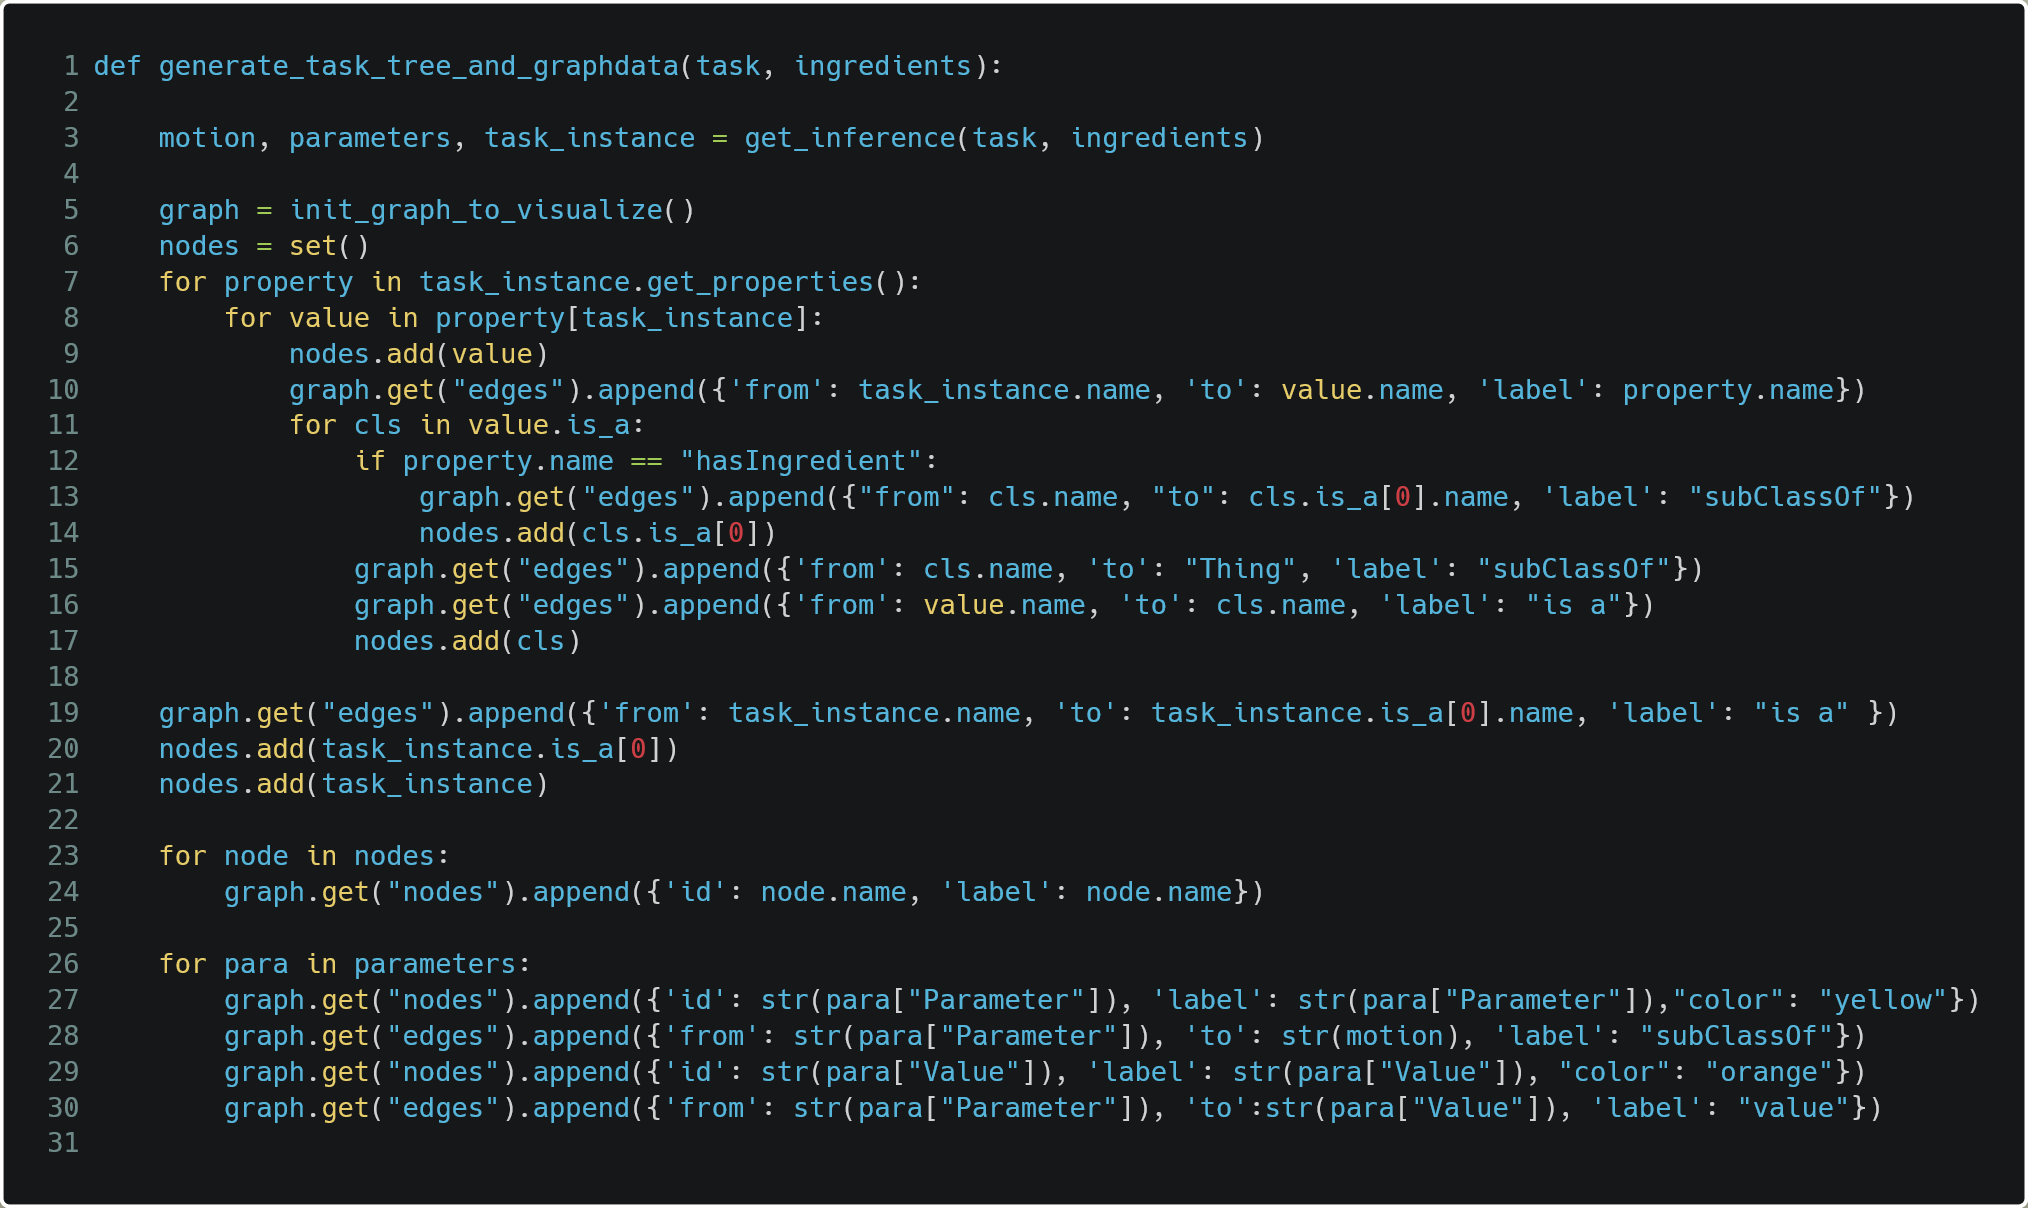
\includegraphics[scale=0.2]{Graphics/get_graph_data_new.png}
    \caption{generating the visualized graph and task tree}
\end{figure}

\begin{itemize}
    \item Line 3: The results of the inference function (see: \nameref{par:Inference}) are stored and used for further processing.
    \item Lines 5 and 6: We initialize an empty graph, which will be filled with nodes and edges throughout the function. Additionally, a set is initialized for the set of nodes.
    \item Lines 7 to 17: Based on the task instance, the graph is structured starting from this node. It checks which relations exist for this instance and accordingly inserts into the set of edges and nodes. Additionally, for the \textit{hasIngredient} relation, the superclass of the ingredient is considered. Finally, the edge labeling is chosen based on the relation, and the classes are added to the graph.
    \item Lines 19 to 21: The task instance itself is processed and added to the graph.
    \item Lines 23 and 24: Iterating over the set of nodes, they are added to the graph.
    \item Lines 26 to 30: The inferred parameters are processed and added to the graph in the end.
\end{itemize}

For the task tree, we create a 3-column table. The first column represents the step, the second column represents the action, and the third column represents the parameters used to illustrate them. The task tree is a list of entries, which can also contain dynamic data such as motions and ingredients.
\begin{figure}[H]
    \includegraphics[scale=0.2]{Graphics/get_graph_data_new2ä.png}
    \caption{generating the visualized graph and task tree}
\end{figure}

\begin{itemize}
    \item 1: The first entry pertains to the robot's action, which is to choose a tool for the upcoming actions. The list of \textit{Tools} corresponds to the subclasses of \textit{Tools} from the ontology. (REFERENCE TO GET TOOLS LEAF)
    \item 2 and 3: Analogous to the first entry, the container is chosen and must be held with an arm for the upcoming motion.
    \item 4: This action describes the starting point of the motion; each motion has its own starting point (see: \nameref{chap:Motions}).
    \item 5: In this step, it is explained with which parameters the motion must be executed.
    \item 6: Once the motion execution is complete, the used tool is set aside.
    \item 7: The final step does nothing but announce the end of the task tree.
    \end{itemize}

These data are forwarded to the frontend via the \textit{flask} interface, where ultimately the graph and the task tree are visualized (see: \ref{fig:graph_inferred})

\section{Fazit}

\subsection{Weaknesses}

\paragraph{Using vis.js}
Using the graph visualization library vis.js yields poor performance on large graphs.
This reason is known to the developers of vis.js (See reference) and the cause of the problem is coming
from the physics simulation. The visualized graph is a force directed graph and the physics simulation attempts to make a user readable graph 
by seperating and clustering nodes who don't or belong to each other. This is done iteratively and consumes a lot of time for large sets of nodes
connected via many edges. The more interconnected the graph is the more terrible the performance gets. 

\paragraph{Data Visualizer}
This framework in its core is not a graph data visualizer. While it is absolutely able to display relationships and attributes of instance data, visualizing 
large datasets defined as ontology is not feasible. It is limited by vis.js which is poorly optimised for large sets of nodes and edges. 
Thus this framework can't be a graph data visualizer. 